\section{Machine Learning Applied to a BSM Search}
So far I have presented the goal of my analysis (to discover new physics)
as well as the tools (\ac{ML}) I will be using to achieve it. In this section
I will discuss how \ac{ML} is applied to the problem as well as how it compares
to traditional methods.
\\
As discussed, I have been presented with two sets of data; the measured collision 
data from \ac{ATLAS} and the simulated \ac{MC} data. The origin of the latter data set 
will not be covered in great detail in this thesis, but it is worth mentioning that 
the simulations are based on \ac{SM} theory. In other words, by comparing the measured collision 
data with the \ac{SM} simulations, we are essentially comparing what is predicted by the \ac{SM} 
to what is measured by experiment. If the two differ in ways not explained by computational error 
or similar, one could interpret the deviation as a new physics.
\\
To summarize, a search for new physics, is a search for deviation between simulation and 
experiment. At first thought, this might seem like a simple task. And if said deviation 
were large, it would be easy. In reality, any new physics which predicts large contributions 
in the data currently measured by \ac{ATLAS} has been excluded a long time ago. Today, any
promising extension of the \ac{SM} predicts to contribute weakly in any detector. As will 
be presented in later section, some theories that will be searched for in this thesis, only 
contribute to a total of 6 events in a data set consisting of more than $3800000$ events 
($<0.002\%$). Not only would such a deviation be incredibly hard to detect, but it would 
be close to impossible to determine if such a deviation is rooted in new physics or simply 
statistical deviation between the two sets of data. 
\\
The traditional approach to this problem, is to study the data in physics motivated regions. 
For example, in section \ref{sec:signal} I presented the feynman diagrams of the signals I 
searched for in this thesis. As mentioned, this type of final state is expected to exhibit 
large amounts of missing transverse energy\footnote{Due to the neutralions being both heavy 
and neutral.}. The traditional approach is to neglect all the data with small amounts of missing 
energy, and only consider events of interest. By applying these kinds of constraints on the data, 
you are creating a region where you expect to find as much of the signal as possible and as little 
of the background. After applying a sufficient amount of demands (or cuts), you would count the 
remaining data in your \emph{search region} and check for deviation. This approach is called cut-and-count.
\\
\begin{figure}
    \centering
    \makebox[0.75\linewidth][c]{%
    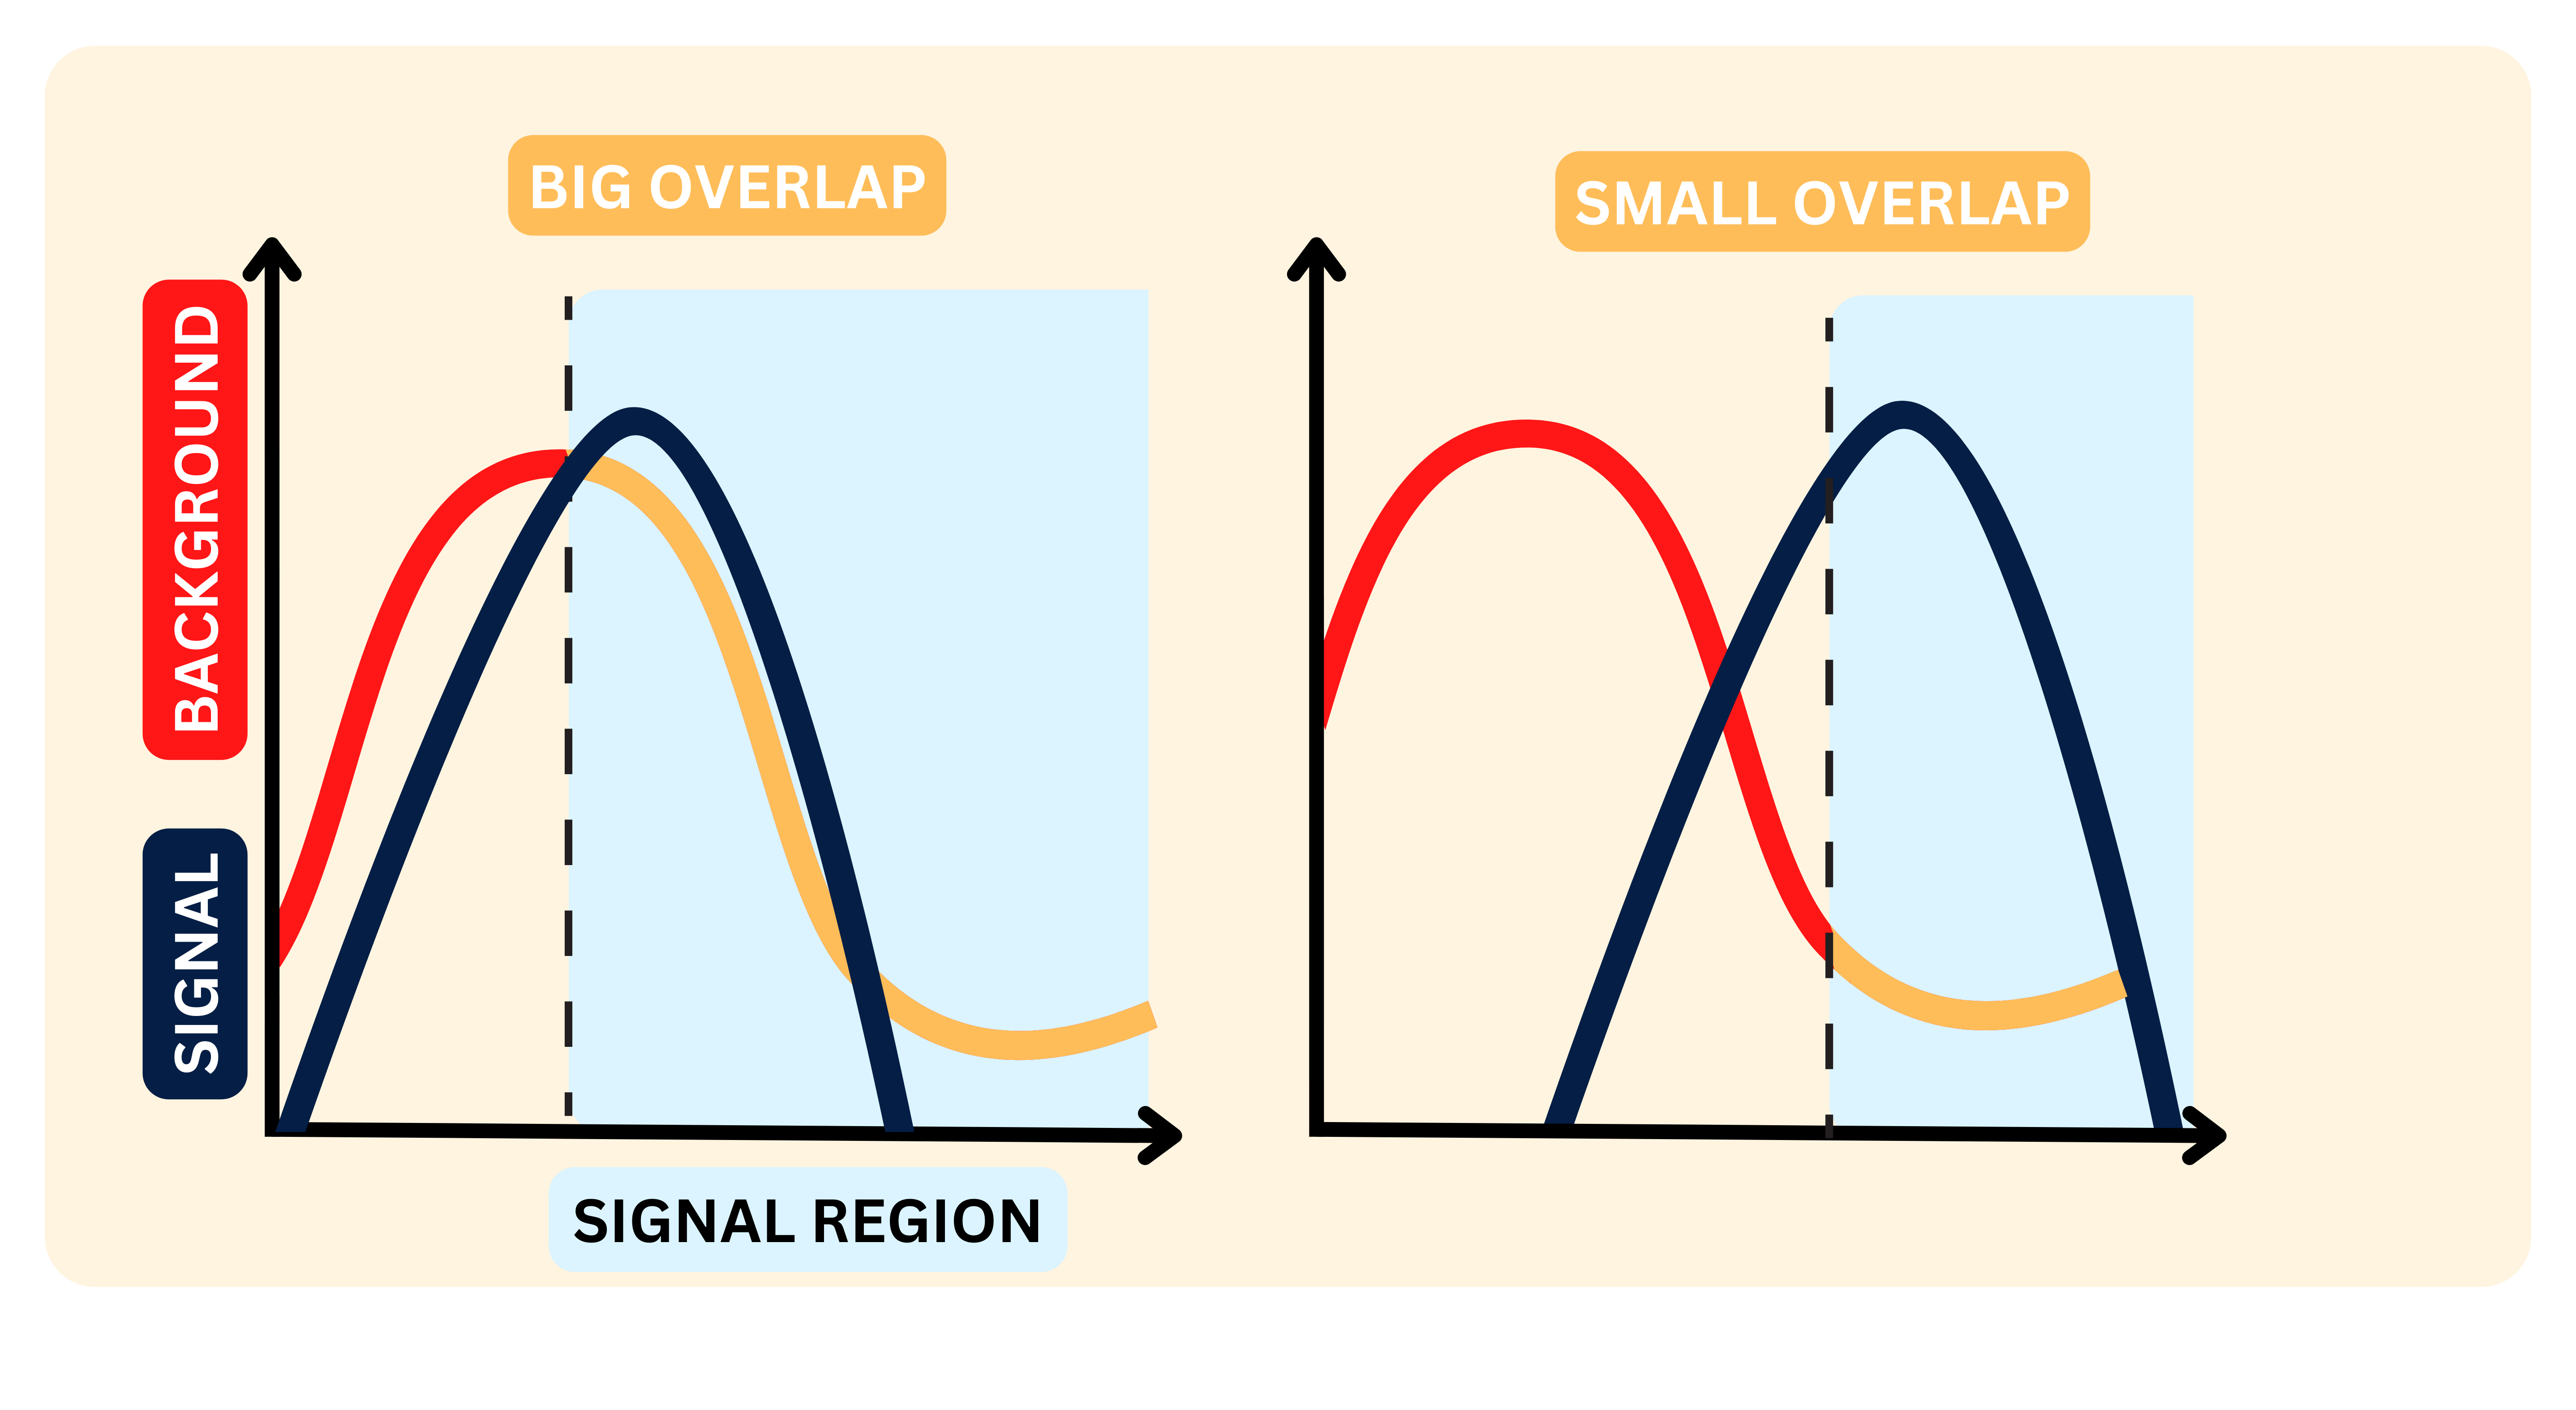
\includegraphics[width=0.65\textwidth]{Figures/Illustrations/CandC.png}
    }
    \caption{An illustration of a traditional cut-and-count approach as well 
    as the motivation for creating a \ac{ML} variable.}
    \label{fig:ROC}
\end{figure}
\subsection{Interpretability}